\section{The Boundary: Priority-Queue Workloads}
\label{sec:negative}

A natural first instinct, given \DeltaSort's $O(n + k\log n)$ comparison bound,
is to apply it to any system that uses a priority queue with batched updates:
A$^*$ and Dijkstra search frontiers, discrete-event simulation queues, OS task
schedulers. We tested A$^*$ with realistic node updates and find that this
instinct is wrong.

The proper baseline is not a sorted array re-sorted on demand, but a binary
min-heap with an explicit \emph{position map} (\PosHeap): an auxiliary array
\texttt{pos[id] = current heap index} that enables $O(\log n)$
\textsc{Decrease-Key} when an item's priority changes. This is the standard
implementation in textbook A$^*$~\cite{cormen}; it is not a research artifact.

\begin{figure}[t]
  \centering
  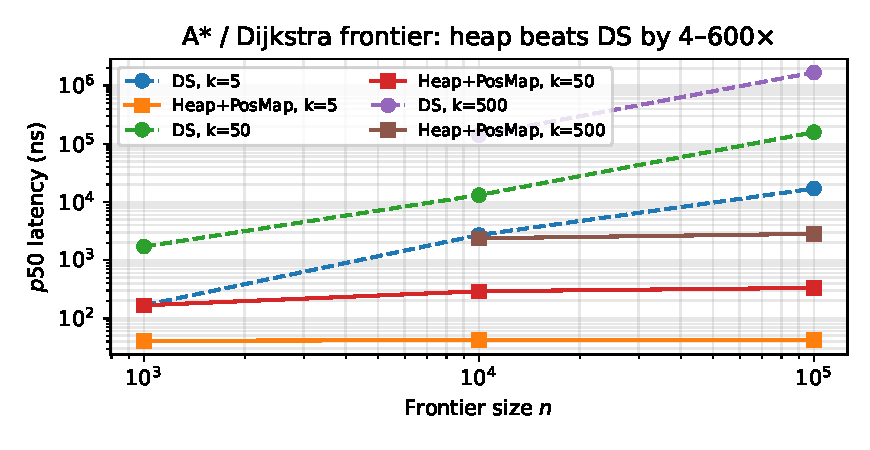
\includegraphics[width=\columnwidth]{figures/negative.pdf}
  \caption{A$^*$ / Dijkstra frontier maintenance: \DeltaSort vs a binary heap
  with explicit position map. Heap is 4--600$\times$ faster across all
  tested $(n, k)$.}
  \label{fig:negative}
\end{figure}

Figure~\ref{fig:negative} shows the comparison. \PosHeap dominates
\DeltaSort by:
\begin{itemize}
  \item $\mathbf{4\times}$ at $n{=}1000$, $k{=}5$,
  \item $\mathbf{64\times}$ at $n{=}10{,}000$, $k{=}5$,
  \item $\mathbf{406\times}$ at $n{=}100{,}000$, $k{=}5$,
  \item up to $\mathbf{599\times}$ at $n{=}100{,}000$, $k{=}500$.
\end{itemize}

The reason is structural: a priority queue only needs the \emph{minimum}
element at any time, never the full sorted order. A heap delivers
$\textsc{Find-Min}$ in $O(1)$ and $\textsc{Update}$ in $O(\log n)$.
\DeltaSort, in contrast, produces the entire sorted array on every batch,
work that is wasted when the consumer only pops the front.

This negative result is decisive and bounds the algorithm's scope. The
characterization is:

\begin{quote}\itshape
\DeltaSort wins when the consumer needs full sorted order (range scans,
top-$k$ with $k$ comparable to $n$, ordered traversal). It loses to a heap
when the consumer only needs the extremum.
\end{quote}

Several otherwise-attractive applications fall on the wrong side of this
line: discrete-event simulation (only the next event matters), OS task
scheduler (only the next task), Dijkstra/A$^*$ search frontier (only the
best node to expand). For these, the textbook heap is and remains the
right tool.

\paragraph{Architectural mismatch: Bevy render phases.}
We also evaluated the Bevy 0.18.1 game engine's transparent render-phase
sort. Initial microbenchmarks against an \texttt{IndexMap}-style baseline
suggested \DeltaSort wins, but production integration revealed a structural
issue: Bevy's \texttt{ViewSortedRenderPhases} are \emph{cleared and
re-extracted every frame} from the ECS world, leaving no persistent sorted
state across frames for \DeltaSort to update incrementally. The current
\texttt{radsort\_by\_key}-on-cleared-buffer pattern is in fact close to
optimal for that architecture. This is not a performance loss but a
structural mismatch: \DeltaSort requires persistent sorted state with known
in-place updates, a precondition this design does not provide.
